Large Language Models (LLMs) have become a cornerstone of modern Natural Language Processing (NLP), enabling a wide range of applications such as chatbot systems, code generation, and content creation: it is estimated that by the end of 2025 there will be 750 million apps using LLMs as a source of interaction. \cite{uspenskyi2025} This chapter provides an overview of current leading LLM families and their innovations, explores key techniques for their customization, introduces the concept of Retrieval-Augmented Generation (RAG), Tool Utilization and Prompt Engineering.


\section{Major Model Families and Their Characteristics}
\label{sec:major-models}

Most LLMs nowadays are built on the Transformer architecture with hundreds of millions to hundreds of billions parameters (and, in recent works, over a trillion), which take advantage of the availability of large-scale text corpora on the internet, along with improvements in scalable hardware (GPUs, TPUs) and advances in Transformer architecture, that adhere to the \textit{scaling law} \cite{kaplan2020scaling} for which systematically scaling model size, data size, and compute lead to improved performance in LLM models. 

Overall, LLMs nowadays can be divided into three main families. \cite{minaee2024largelanguagemodelssurvey}


\subsection{GPT Family (Generative Pre-Trained Transformers)}

The GPT family consists of decoder-only models developed by OpenAI, introducing GPT in 2018, which is defined as an undirectional auto-regressive model. The key innovation here is that it showed that large-scale, unsupervised pre-training followed by a punctual fine-tuning on specific tasks that the model is supposed to achieve, could outperform traditional architectures of many NLP benchmarks.

A year later, the company introduced GPT-2, scaling up the parameter count up to 1.5 billion parameters: it demonstrated zero-shot capabilities on tasks like summarization or translation, only using prompting for interacting with the model.

The term \textit{zero-shot capability} refers to the ability for a model to prompting an LLM without any examples, attempting to take advantage of the generalization it has gained through training, using reasoning patterns it has acquired.

GPT-3 saw another scale up in parameters count, achieving a surprising 175 billion count: by giving few-shot examples at inference time, it demonstrated an \textit{in-context learning}, for which no additional fine-tuning was required.

Finally, GPT-3.5 introduced the renowned \textit{ChatGPT}, which introduced LLMs to the general public. It incorporated instruction-following behavior and Reinforcement Learning from Human Feedback (RLHS) to reduce harmful content; later, with GPT-4, it introduced multi-modal capabilities interacting with and generating non-textual data.

Overall, the GPT Family has been acclaimed for its investments in scaling models with higher parameters and text corpora, achieving few-shot capabilities without the need to further training models.


\subsection{BERT Family (Bidirectional Encoder Representations)}

The BERT-family was introduced by Google in 2018, and it focuses on tasks that require understanding of the input, such as sentence classification and named entity recognition. In this context they utilize and encoder-only architecture, performing a masked contextual understanding, meaning that their training in based mainly on masking tokens at each iteration and gaining a probabilistic choice of the next token prediction.

This kind of models are strong at understanding the semantics of text from a bidirectional perspective: through Masked Language Modeling (MLM), the training consists of randomly masking 15\% of the tokens in the input and ask the model to predict the original vocabulary tokens, encouraging to learn from the left and from the right sides of the masked token (that is, bidirectional).

BERT is by design a 110 million parameters in its base version, whereas it has 340 million parameters in its largest one, which has seen several variants over the years, like RoBERTA which increased training data and steps involved in the training phase, or ALBERT, with a parameter-reduction technique to handle scaling more efficiently, and finally DistilBERT, that implemented \textit{knowledge distillation}: a novel technique in making LLMs more practical and efficient, by transferring essential knowledge from a complex teacher model to a smaller student model, preserving performance while reducing size and computational demands.


\subsection{T5 Family (Text-to-Text Transfer Transformer)}

Introduced as well by Google (2019), the T5-family model uses a full sequence-to-sequence (i.e., encoder-decoder) Transformer architecture. The core idea is to formulate every NLP task as a "text-to-text" problem-inputs and outputs are always text strings.

Prior to T5, large-scale models (e.g., GPT, BERT) had shown the power of pre-training on unlabeled data followed by task-specific fine-tuning; however, these approaches often frame tasks differently (classification vs prediction vs language modeling). This divergence complicates the use of a single frameworks for multiple tasks: so, the goal was to create a unified approach to NLP tasks by casting all problems into a text-to-text format.

The authors released multiple variants, with the largest size counting up to 11 billion parameters, and their approach in training was a modified version of MLM, which is Span Corruption: randomly masking not individual tokens, by entire span of texts. This demonstrated to foster a more coherent learning of consecutive tokens and encouraged the model to handle variable-length contexts.

The T5 has been superseded later on by mT5 and T5-XXL, with larger parameter counts and multilingual corpora for cross-lingual transfer, which yields strong results across different tasks, highlighting flexibility for multitask settings.

These families do not comprise the several hundreds of foundation models released in recent years, but it nonetheless give a high perspective of the model architectures, their characteristics and key innovations. A common strategy has been underlined across the realm of these families: the bigger the size, the better. That is why training has always been a prerogative of the few, large companies or research centers that can handle higher computational resources and costs.


\section{Beyond Fine-Tuning: Alternative Strategies for Optimizing LLMs}

Given the computational challenges of fine-tuning, alternative approaches such as Retrieval-Augmented Generation (RAG), Prompt Engineering, and Agent AI have emerged as effective strategies for achieving task-specific accuracy without the need for extensive model retraining.

As LLMs become increasingly prevalent, practitioners have devised a range of methods to tailor their behavior for specific use cases and to deploy them efficiently. Fine-tuning remains a common approach, allowing developers to update the model weights on domain-specific datasets. This can be performed as a full-scale process, adjusting all parameters, or via more parameter-efficient methods such as \textit{LoRA}, \cite{hu2021lora} which inserts low-rank updates into the model’s layers and thus reduces memory requirements; this approach still produces prohibitive settings to develop LLM specific implementations, that is why innovative techniques have emerged, gathering fine-tuned models that possess general knowledge directing its focus on specific tasks and use cases.

Prompt engineering, takes advantage of the model’s pre-trained knowledge by carefully crafting textual instructions that guide it toward the desired output. \cite{liu2023promptsurvey} Rather than modifying the model weights, prompt engineering modifies the input context to clarify the task objective or to showcase example queries and answers. This practice has grown in importance with the rise of instruction-tuned models, which are trained to follow natural language instructions rather than purely statistical patterns.

Another pivotal approach involves integrating an external knowledge base into the generation process. Retrieval-Augmented Generation (RAG) \cite{lewis2020retrieval} leverages a retrieval module, typically built on vector search engines, to fetch relevant documents or snippets from a corpus. The LLM then conditions its output on these retrieved texts, thereby grounding its responses in verifiable sources and reducing hallucination or factually incorrect statements. \cite{ji2023surveyhallucination}

Lastly, the concept of Tools have introduced the term "AI Agents". Tools are external modules or functions that the model can decide to invoke, to perform tasks or gather knowledge which was not comprised in its training and go beyond text generation. It leverages the model's internal decision mechanism that will determine if an action must be taken based on users' input. For example, asking what the weather is like right now is excluded by the factual limited knowledge the model possesses; it can be thereby create a tool that calls an API with weather data, and when the trigger has been captured by the model it can decide to call this tool to retrieve the updated data.

In the next sections we will dive into these innovative strategies to benefit from pre-trained models with powerful text-generation abilities of LLMs without incurring into expensive setups. Nevertheless, it must be first introduced the concept of prompting and the interaction with a language model.


\subsection{From Words to Numbers and Back to Words: Tokenization}
\label{sec:tokenization}

\textit{Tokenizers} are one of the core components of the NLP pipeline, which hey serve one purpose: to translate text into data that can be processed by the model. As in language models the data that is generally produced is raw text, and knowing that Transformers can only process numbers, tokenizers need to convert text inputs to numerical data. So, the goal of tokenizers is to find the most meaningful representation — that is, the one that makes the most sense to the model — and if possible the smallest representation.

Tokenization splits text into manageable units (that is, \textit{tokens}) to enable the model to understand and process language, which are then converted into numerical representations that capture their semantics. It can be as simple as a word-based tokenization (i.e., each word is a token), to more complex techniques like \textit{WordPiece} used in BERT models.

Each token is defined by the method used, for which the first that comes to mind would be a word-based tokenization. As an example, having the phrase "John was a puppeteer" could be divided into

\begin{verbatim}
    Jim | Henson | was | a | puppeteer | .
\end{verbatim}

And the goal would be to assign a numerical representation of each token

\begin{verbatim}
    Jim | Henson | was | a | puppeteer | .
    545 | 4668   | 109 | 9 | 10988     | 721 
\end{verbatim}

Each word gets assigned an ID, starting from 0 and going up to the size of the vocabulary: then the model uses these IDs to identify each word. But if we want to completely cover a language with a word-based tokenizer, we’ll need to have an identifier for each word in the language, which will generate a huge amount of tokens. For example, there are over 500,000 words in the English language, so to build a map from each word to an input ID we’d need to keep track of that many IDs. Furthermore, words like “dog” are represented differently from words like “dogs”, and the model will initially have no way of knowing that “dog” and “dogs” are similar: it will identify the two words as unrelated. The same applies to other similar words, like “run” and “running”, which the model will not see as being similar initially. \cite{huggingfacecourse}

Other simple tokenization techniques could come to mind, for example a character-based tokenization, but the reality would be very complex and could not tackle the semantics of the context. Several techniques have been developed, of which the most important are: \cite{rajaraman2024theorytokenizationllms}

\begin{itemize}
    \item \textbf{Byte-Pair Encoding (BPE):} Used by models like GPT-2 and GPT-3, BPE starts with individual characters and iteratively merges the most frequent pairs to form subwords. This helps manage vocabulary size and handle rare or novel words. \cite{sennrich2016neural}
    \item \textbf{WordPiece:} Employed by BERT, WordPiece is similar to BPE but merges tokens by maximizing the likelihood of token sequences. It helps capture the structure of language by efficiently splitting words into meaningful subword units.
    \item \textbf{SentencePiece:} Often used in models like T5, SentencePiece does not rely on pre-tokenized input. It treats the text as a raw sequence of characters (or bytes) and learns subword units directly, making it versatile across languages and scripts.
\end{itemize}

The process of extracting meaning from raw text to discrete representation and then back to words can be seen in Figure \ref{fig:tokenization}.

\begin{figure}[b]
    \centering
    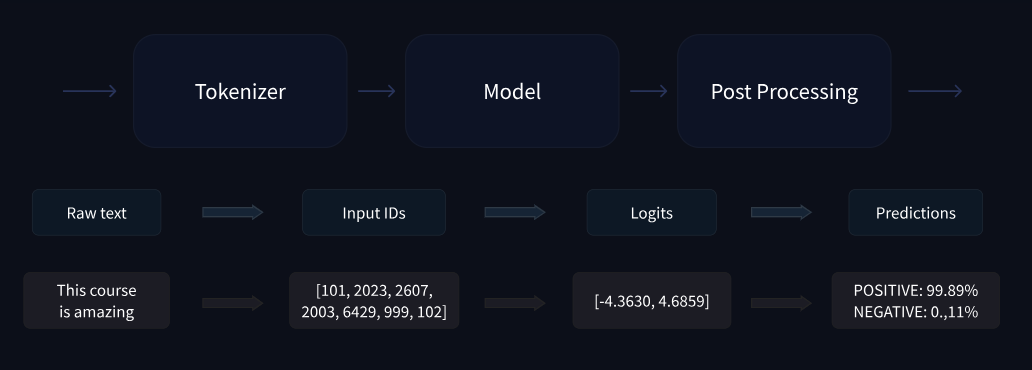
\includegraphics[width=1\textwidth]{images/tokenizer-process.png}
    \caption{The tokenization process referring to text classification, as seen in \cite{huggingfacecourse}.}
    \label{fig:tokenization}
\end{figure}

Translating text to numbers is known as \textit{encoding} (not to be confused with \textbf{encoders} in the Transformer architecture). Encoding is done in a two-step process: the tokenization, followed by the conversion to input IDs, of which the set of all possible IDs is called a \textit{vocabulary} of the model that learned during the training phase.

Each input ID is then converted into a high-dimensional vector that represents the contextual understanding of that input by the Transformer model. The subsequent layers of the architecture manipulate those vectors using the attention mechanism to produce the final representation of the sentences. \cite{vaswani2017attention}

The model outputs logits for each position in the sequence (for language modeling, this is typically predicting the next-token distribution): logits are real-valued scores for each token in the vocabulary before activation.

These scores are then converted to probabilities, yielding a probability distribution over the vocabulary for the next token to predict through a \textit{SoftMax} layer

\[
\text{Logits} = [1.3, 5.1, 2.2, 0.7, 1.1]
\]
\[
\text{Softmax}(z_i) = \frac{e^{z_i}}{\sum_{j=1}^{K} e^{z_j}}
\]
\[
\text{Probabilities} = [0.02, 0.90, 0.05, 0.01, 0.02]
\]

which turns logit scores into probabilities.
Finally, the \textit{decoding} phase chooses the tokens to output, for which a few strategies could be adopted: \cite{radford2018improving}

\begin{itemize}
    \item \textbf{Greedy Decoding (Argmax)}: Choose the token with the highest probability at each step.
    \item \textbf{Beam Search:} Maintain multiple candidate sequences to reduce the chance of missing higher probability sequences.
    \item \textbf{Sampling:} Randomly sample from the distribution to introduce diversity.
    \item \textbf{Top-k/Top-p Sampling:} Limit sampling to the top-k most probable tokens or cumulative probability p, improving coherence and variety.
\end{itemize}

The predicted token IDs are finally mapped back to subwords or tokens via the tokenizer's vocabulary, and subwords are joined or merged to form readable text.





\subsection{Anatomy of a Prompt}
\label{sec:prompt-anatomy}

A \textbf{prompt}, sometimes referred to as context, is the text provided to a model before it begins generating output; it guides the model to explore a particular area of what it has learned so that the output is relevant to the prefixed tasks. Frequently, prompts will be an instruction or a question:

\begin{Verbatim}[breaklines=true]
Question: Explain the theory of gravity to a 6 year old.
Answer: Gravity is like a big invisible hug that pulls everything down. It's like an invisible rope that connects everything in the world, and it pulls things closer together. When you jump yp in the air, gravity pulls you back down to the ground. That's why you can't just fly away!
\end{Verbatim}

In applications where a user is interacting with a model dynamically, such as chatting with the model, there will typically be portions of the prompt that are never intended to be seen by the user. These hidden portions may occur anywhere, though there is almost always a hidden prompt at the start of a conversation.
Typically, this includes an initial chunk of text that sets the tone, model constraints, and goals, along with other dynamic information that is specific to the particular session--user name, location, time of day..

The model is static and frozen at a point in time, so if the user wants the model to know current information, as for example time or weather, it must be provided to the model itself.

A common standard in chat models has been delineated by OpenAI, for which a categorization of roles has emerged from empirical design choices in conversational AI systems (namely, ChatGPT), where:

\begin{enumerate}
    \item \textbf{System:} Sets the overall context, rules, and instructions that govern the conversation. It provides the “hidden” guidelines the assistant follows to ensure responses are consistent with desired policies, style, and behavior.
    \item \textbf{User:} The user is the one providing the queries, prompts, or instructions that drive the conversation. Their input defines what information or assistance is being requested, and the assistant responds accordingly.
    \item \textbf{Assistant:} This is the language model’s persona that generates responses based on the system instructions and user inputs. The assistant’s job is to provide helpful, accurate, and context-aware answers while adhering to the guidelines set by the system.
\end{enumerate}

Guidelines can be found in OpenAI's documentation, following Table \ref{tab:roles}. For example, a conversation following the aforementioned roles could be:

\begin{Verbatim}[breaklines=true]
\underline{SYSTEM}:     You are a helpful assistant that answers programming questions in the style of a southern belle from the southeast United States.

\underline{USER}:       Are semicolons optional in JavaScript?

\underline{ASSISTANT}:  Well, sugar, that's a fine question you've got there! Now, in the world of JavaScript, semicolons are indeed a bit like the pearls on a necklace, you might slip by without 'em, but you sure do look more polished with 'em in place.
Technically, JavaScript has this little thing called "automatic semicolon insertion" where it kindly adds semicolons for you where it thinks they oughta go.
However, it's not always perfect, bless its heart.
Sometimes, it might get a tad confused and cause all sorts of unexpected behavior.
\end{Verbatim}

It can be noted that the use of the message types above to provide additional information to the model outside of its training data has spiked an answer in the style requested by the context.
The idea of role prompting is rooted in the broader literature on prompt engineering and instruction tuning, and several strategies have been developed in order to make the most out of prompting. \cite{openai2025textgeneration}

\begin{table}[hb]
    \centering
    \renewcommand{\arraystretch}{1.3}
    \begin{tabularx}{\textwidth}{|X|X|X|}
        \hline
        \textbf{Role} & \textbf{Description} & \textbf{Usage example} \\
        \hline
        \textbf{user} &
        Instructions that request some output from the model. Similar to messages you'd type in ChatGPT as a user. &
        \textit{Write a haiku about programming.} \\
        \hline
        \textbf{system} &
        Instructions to the model that are prioritized ahead of user messages, following chain of command. Previously called the system prompt. &
        \textit{Describe how the model should generally behave and respond.} \\
        \hline
        \textbf{assistant} &
        A message generated by the model, perhaps in direct response to the current request. &
        \textit{For example, to get the model to respond correctly to knock-knock jokes, you might provide a full back-and-forth dialogue of a knock-knock joke.} \\
        \hline
    \end{tabularx}
    \caption{Examples of Instruction Tuning}
    \label{tab:roles}
\end{table}




\section{Prompt Engineering}
\label{sec:prompt-engineering}

Prompt engineering is defined as the process of designing and structuring instructions (prompts) to guide LLMs toward producing the most effective outputs without modifying the models’ internal parameters. In this context, a prompt is more than just a query—it’s a carefully crafted input that may include context, instructions, role definitions, and even examples to help the model understand the desired task. \cite{sahoo2024systematicsurveypromptengineering}

Several techniques have been demonstrated to enhance models' performance in various tasks, with regard to increasing model sizes. \cite{brown2020language}


\subsection{In-Context Learning}
\label{sec:in-context-learning}

When interacting with a language model, we usually ask a question or give a command in general. The same question asked or instruction given generate a different response each time, as the determinism of the response itself is not guaranteed due to the stochastic nature of the Transformers output. At the same time, questions or instructions given in different ways returns different responses: providing examples of the task we are trying to carry out is called \textbf{In-Context Learning}.

In-Context Learning refers to the ability of a language model to perform new tasks by leveraging examples provided directly within the prompt, rather than through explicit parameter updates. The model infers the underlying task by observing a set of input-output pairs included in the prompt and then generalizes that pattern to generate a response for a new input. This process effectively allows the model to "learn" from context during inference time.

When a language model is given a task instruction without any example inputs or outputs, relying solely on its pre-trained knowledge and the explicit prompt, it is referred as \textit{Zero-Shot Prompting}.
It tests the model’s ability to generalize to tasks it was never explicitly trained on, solely by interpreting the instruction given in natural language. For example,

\begin{Verbatim}[breaklines=true]
\underline{USER}:       Message: Hi Amit, I loved my birthday card!
             Sentiment:
\underline{ASSISTANT}:  Sentiment: Positive. 
\end{Verbatim}

Here the task is to classify the sentiment of the sentence provided. It does not include any example on how to achieve the result, any hint on how to interpret the task or how to format it. Zero-Shot is not always performant, especially in low-rank parameters models, as shown in Figure \ref{fig:prompting-accuracy}.

\begin{figure}[h]
    \centering
    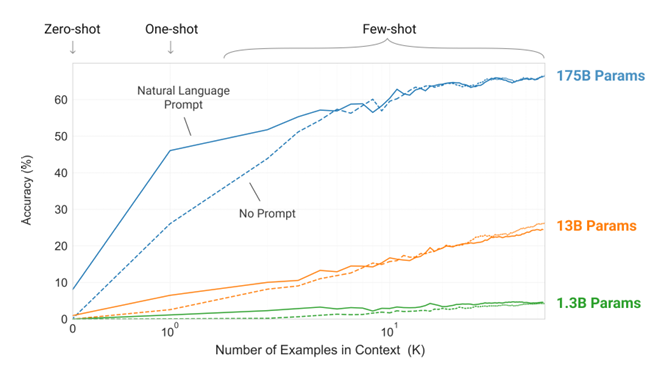
\includegraphics[width=0.7\textwidth]{images/accuracy-prompting-techniques.png}
    \caption{Different prompting techniques can increase models' accuracy, as seen in \cite{brown2020language}.}
    \label{fig:prompting-accuracy}
\end{figure}

Providing examples can help the model to understand the task:

\begin{Verbatim}[breaklines=true]
    USER        Message: Dad, you are 20 minutes late for my piano recital!!
                Sentiment: Negative
                Message: Hi Amit, I loved my birthday card!
                Sentiment:
    ASSISTANT   Sentiment: Positive.
\end{Verbatim}

Giving the model an example, and then the task we want it to perform is called \textit{One-Shot Prompting}; two or more examples given to the model is called \textit{Few-Shot Prompting}. As shown in Figure \ref{fig:prompting-accuracy}, increasing the number \textit{k} of examples along with the increasing number of parameters held by the model's architecture improve task accuracy.


\subsection{Chain-of-Thought}
\label{sec:cot-prompting}

\textbf{Chain-of-Thought} is a novel method to enhance the reasoning capabilities of large language models by encouraging them to generate intermediate steps—what the authors call a "chain of thought"—before arriving at a final answer. \cite{wei2023chainofthought}

This technique allows models to decompose multi-step problems into intermediate steps, suggesting how it might have arrived at a particular answer and providing opportunities to debug where the reasoning path went wrong; it has been demonstrated to be useful for tasks such as symbolic manipulation, commonsense reasoning and arithmetic problems, as can be seen in \ref{fig:cot-prompting}, where the Chain-of-Thought reasoning process is highlighted compared to standard prompting.

\begin{figure}[h]
    \centering
    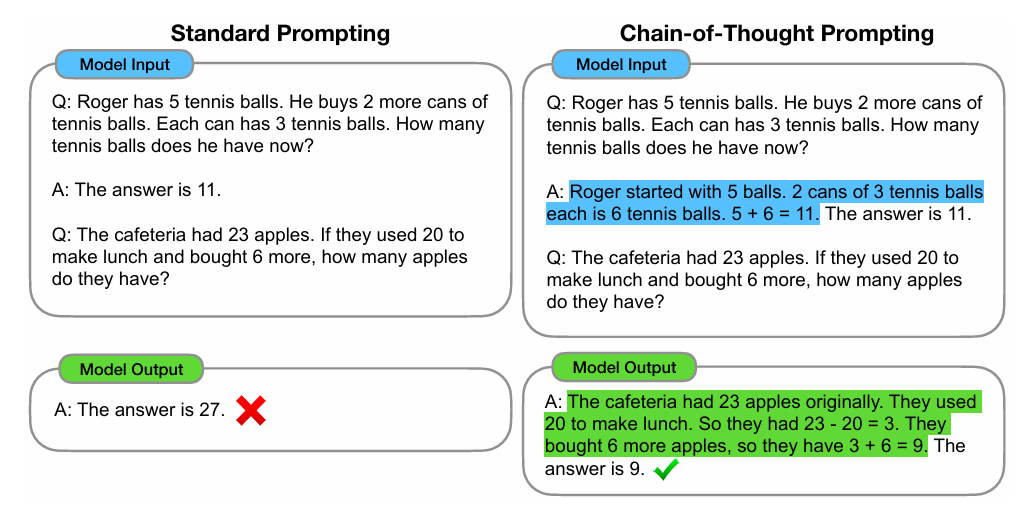
\includegraphics[width=0.7\textwidth]{images/cot-prompting.png}
    \caption{Standard prompting compared to Chain-of-Thought prompting, as seen in \cite{wei2023chainofthought}.}
    \label{fig:cot-prompting}
\end{figure}

Traditional prompting methods typically ask the model to produce an answer directly, but when it comes to multi-step reasoning task-as the simple arithmetic problem in Figure \ref{fig:cot-prompting}-this approach often fails. This is why guiding the model to reason through intermediate steps can lead to improved performance because, instead of forcing the model to output a single-step response, one can prompt it to "think out loud" by generating a sequence of reasoning steps. This simulates a human-like problem-solving process, where intermediate calculations or logical steps are made explicit before reaching a conclusion.


\subsection{Role Prompting}
\label{sec:role-prompting}

\textbf{Role Prompting} is the practice of explicitly instructing a language model to adopt a specific persona or role within the prompt. By doing so, the model is provided with contextual cues about the kind of responses expected. For example, a prompt might begin with "You are an expert financial analyst," which sets the stage for subsequent output to be informed by that role. This approach leverages the model’s vast pre-trained knowledge while narrowing its focus to the style, tone, and depth that a particular role implies. \cite{reynolds2021promptprogramminglargelanguage}

Framing the task in a way that aligns with the attributes of the designed role, can lead to more coherent and contextually appropriate responses, as the model "activates" a domain-specific language pattern and knowledge; when a model is prompted with a clear role, its output tend to be better aligned with the requirements. Just think of an assistant in medical or judicial domain, must adhere to a specific language and adapt itself to the context involved. To appreciate the different results produced by different roles can be seen in the following demonstration: \cite{w3schools2025}

Acting as a lawyer:
\begin{Verbatim}[breaklines=true]
\underline{USER}:       You are a Lawyer. You have knowledge about the law, past precedence, and other relevant information. Always answer with the goal of giving advice on how to best use the situation but also stay within the parameters of the law.
Respond to the following:
"Explain the most important way ChatGPT can help me. The answer should be no more than 100 words."
               
\underline{ASSISTANT}:  As a lawyer, I understand the importance of providing concise and clear advice to my clients. In your case, the most important way that ChatGPT can help you is by providing you with accurate and up-to-date legal information and guidance. ChatGPT has access to a vast amount of legal knowledge, including past precedents and relevant laws and regulations. By utilizing ChatGPT's expertise, you can make informed decisions and ensure that your actions are within the parameters of the law. Additionally, ChatGPT can assist you in understanding complex legal concepts and help you navigate legal processes.
\end{Verbatim}

Acting as Yoda:
\begin{Verbatim}[breaklines=true]
\underline{USER}:       You are Yoda from "Star Wars". You have all the knowledge of Yoda. Answer like Yoda using the manner of speaking and vocabulary of Yoda.
Respond to the following:
"Explain the most important way ChatGPT can help me. The answer should be no more than 100 words."
               
\underline{ASSISTANT}:  Help you, ChatGPT can, in many ways. But most important, it is to expand knowledge and wisdom, hmm? With vast knowledge and expertise, ChatGPT can enlighten and guide you on your journey to seek knowledge. Questions, you have? Ask, ChatGPT will answer. Advice, you seek? Seek, ChatGPT will offer. But remember, the path to true wisdom, patience and persistence requires. Patience, you must have, young one. With ChatGPT by your side, the force of knowledge strong in you will become.
\end{Verbatim}

Role Prompting is thus very useful for setting the tone and the context of the conversation, preserving model parameters and general knowledge. But a model's knowledge ends at the moment of its training - so it will not know about more recent events, current literature or real-time information: in \ref{sec:rag} a novel technique is discussed for injecting specific knowledge into a language model.



\section{Retrieval Augmented Generation}
\label{sec:rag}

LLMs have proven to be powerful few-shot learners, \cite{brown2020language} able to learn and execute new tasks, process complex information and solve real problems. However, due to their limited knowledge, the training constraints them to past knowledge, making it difficult to rely on real-time data consumption.

\textbf{Retrieval-Augmented-Generation} (RAG) combines the strength of a retrieval system and generative models to tackle knowledge-intensive tasks, such as open-domain and question answering. In fact, many NLP tasks require access to up-to-date knowledge or data, which can not be retrieved from the training corpora.
It is an approach that enhances a generative model by incorporating external, contextually relevant information into its response process.
In its simplest form, this can involve injecting specific knowledge directly into the system prompt, as briefly introduced in Section \ref{sec:prompt-anatomy}, such that the model first retrieves specific information from an external source and then uses it to generate a more accurate output.

In its original framework, this method combines a \textit{retriever} component, typically based on dense representations of the external source (oftentimes document pools, or a database), enabling efficient similarity search through embedding that include nearest-neighbor search.

\begin{figure}[h]
    \centering
    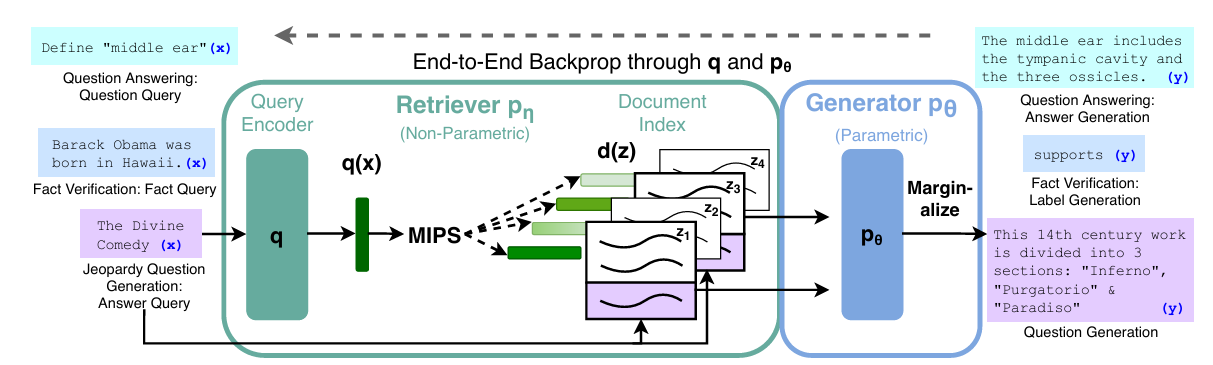
\includegraphics[width=0.7\textwidth]{images/rag-components.png}
    \caption{RAG architecture, as seen in \cite{lewis2020retrieval}.}
    \label{fig:rag}
\end{figure}

Figure \ref{fig:rag} shows the original architecture, which is composed by:

\begin{itemize}
    \item \textbf{Document Corpus:} A large, pre-indexed collection of documents that the retriever searches.
    \item \textbf{Retriever:} This component receives the standard prompt in input (query) and converts it into a representation that can be compared to the dense vector index representation of the document corpora to efficiently locate relevant information.
    \item \textbf{Generator:} The model implemented, which receives the relevant information gained by the retriever and integrates it in its output.
\end{itemize}

Together, these components enable the RAG framework to dynamically integrate specific, contextually relevant knowledge into the generation process, leading to more informed and accurate outputs; nonetheless, in Section \ref{sec:agent-ai} is discussed another technique that allow models to dynamically fetch relevant information via external tools.




\section{Agent AI}
\label{sec:agent-ai}

LLMs have demonstrated to be masters of language and, in recent literature, reasoners capable of answering complex questions and solving problems. But beneath their linguistic brilliance lies a fundamental limitation: they lack autonomy and, as stressed before, are limited by their training data. This is where the concept of agents comes into play: an \textbf{Agent} is a system that leverages an AI model to interact with its environment in order to achieve a user-defined objective. It combines reasoning, planning and executing actions, extending the capabilities of LLMs enabling them to act autonomously via external tools to fulfill a task.

\begin{figure}[h]
    \centering
    \begin{minipage}{0.45\textwidth}
        \centering
        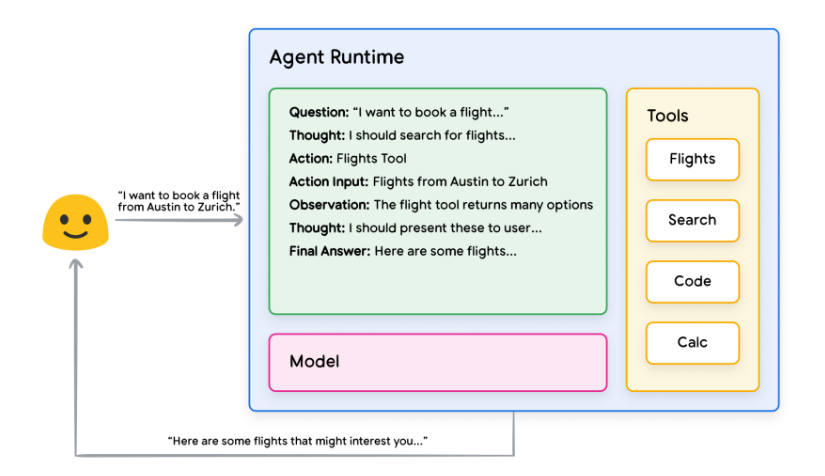
\includegraphics[width=\textwidth]{images/agents.png}
        \caption{An end-to-end agentic behavior.}
    \end{minipage}
    \hfill
    \begin{minipage}{0.45\textwidth}
        \centering
        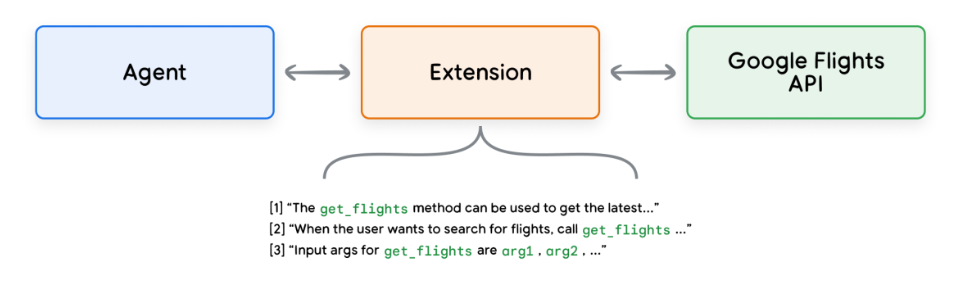
\includegraphics[width=\textwidth]{images/agents-ii.png}
        \caption{The connection from the agent to the external source.}
    \end{minipage}
    \caption{An agent workflow.}
    \label{fig:agent-ai}
\end{figure}

The fundamental component of an Agent is the concept of \textit{tool}: a user-defined function that is integrated in the model which can decide to use if a call-to-action is triggered. For example, in Figure \ref{fig:agent-ai} depicts a simple agentic flow:

\begin{enumerate}
    \item A set of tools is defined: these can vary from call to external APIs to user-defined functions that are run on the clients' environment. In the example above, the focus is on the \textit{Flights} tool, which can perform an API call to Google Flights service in order to retrieve flight attendance, and it is defined by the function \verb|get_flights|.
    \item The model is made aware of the available set of tools, and it is taught when to call them through \textit{few-shot} example as seen in Section \ref{sec:in-context-learning} on how to use them or by a \textit{Chain-of-Thought} approach as seen in Section \ref{sec:cot-prompting}, dissecting the steps required to achieve the task. A simple yet effective prompt could be:
    
    \begin{Verbatim}[breaklines=true]
    The get_flights method can be used to get the latest flight information from the Google Flights service. When the user wants to search for flights, call the function get_flights. Input arguments are "departure", "destination", "date".
    \end{Verbatim}

    \item When the user prompts "I want to book flight from Austin to Zurich", the model activates the orchestration layer which is a cyclical process that governs how the agent takes in information and performs internal reasoning. The model thus uses that reasoning to inform its next action the cognitive architecture section: usually some triggers activate internal reasoning, for example the word "flight" or "book a flight". The agent then starts a multi-step process that calls the function \verb|get_flights| with the captured parameters \verb|"departure": "Austin", "arrival": "Zurich"|. The function is run, the returned result is parsed by the model itself which in turn generates the response to users' prompt.
    Note that tool calling is an actual output, which is different from a straightforward usual response, and it is generally hidden. The input-output sequence:
        \begin{Verbatim}[breaklines=true]
            INPUT     Prompt.
            OUTPUT    Tool: get_flights. Parameters: "departure": "Austin", "arrival": "Zurich"
            INPUT     Call function get_flights with parameters "departure": "Austin", "arrival": "Zurich"
            OUTPUT    Function returned flights.
            INPUT     Present the results flights from Austin to Zurich.
            OUTPUT    "Here are some flights that might interest you..."
        \end{Verbatim}
    The first input is the user's prompt, it then follows the model's output which is not displayed, but instead parsed internally, deciding to use the tool. The function is then run, the result returned and again parsed. Finally, the output is shown, answering the initial prompt.
\end{enumerate}

Agentic framework is gaining remarkable success due to the extensions that calling external tools can provide to a basic model, in particular with regard to image generation, web search and collaborative writing, taking advantage of increasing model sizes and consequently in-context learning abilities, cognition and internal reasoning.